% ═══════════════════════════════════════════════════════════════════════════
% Chapter 4: Hardware Design
% ═══════════════════════════════════════════════════════════════════════════

\chapter{Hardware Design} \label{chap:hardware}

\section{IMU Subsystem}

\subsection{ICM-42688-P Pinout and Interface}

The ICM-42688-P is housed in a 3x3x0.9 mm QFN-24 package. The primary interface for this application is SPI3 (3-wire) operating at 10 MHz:

\begin{table}[h]
    \centering
    \caption{ICM-42688-P critical pins}
    \label{tab:imu_pins}
    \begin{tabular}{lll}
        \toprule
        \textbf{Pin} & \textbf{Name} & \textbf{Function} \\
        \midrule
        1 & VDD & 1.8 V supply (IMU core) \\
        2 & VDDIO & 1.8-3.3 V I/O supply \\
        3 & ASSTA & Active high reset / arming \\
        4 & nCS & Chip select (SPI) \\
        5 & SCLK & Serial clock (SPI) \\
        6 & SDI & Serial data in (SPI) \\
        7 & SDO & Serial data out (SPI) \\
        12 & FSYNC & Frame sync input (hardware timestamp) \\
        15 & INT1 & Data ready interrupt \\
        18 & GND & Ground \\
        \bottomrule
    \end{tabular}
\end{table}

\subsection{Register Configuration}

The sensor is configured via the following register write sequence after reset:

\begin{lstlisting}[caption={ICM-42688-P initialization sequence}, language=c]
// Device configuration (0x01)
WRITE_REG(0x06, 0xB0);  // Soft reset

// Power configuration (0x4E)
WRITE_REG(0x4E, 0x00);  // Wake up

// Gyro configuration (0x3F)
WRITE_REG(0x3F, 0x04);  // 2000 dps, 333 Hz OC, 1000 Hz LPF

// Accel configuration (0x40)
WRITE_REG(0x40, 0x04);  // 16g, 1 kHz OC, 450 Hz LPF

// Interrupt configuration (0x0F)
WRITE_REG(0x0F, 0x02);  // INT1 = Data Ready (active high)

// nero configuration (0x3E)
WRITE_REG(0x3E, 0x20);  // FSYNC enabled, negative logic
\end{lstlisting}

The 1 kHz output data rate (ODR) is achieved with 450 Hz low-pass filter, satisfying Nyquist for weightlifting dynamics (expected bandwidth <200 Hz based on biomechanical studies).

\subsection{Decoupling and Power Delivery}

Each supply pin requires local decoupling within 2 mm:

\begin{figure}[h]
    \centering
    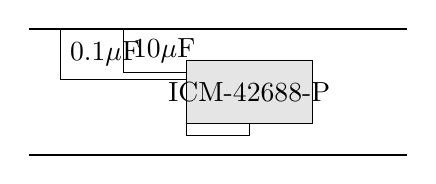
\begin{tikzpicture}[scale=0.8]
        % Power rail
        \draw[thick] (0,2) -- (6,2);
        \draw[thick] (0,0) -- (6,0);

        % IMU symbol
        \draw[fill=gray!20] (2.5,0.5) rectangle (4.5,1.5);
        \node at (3.5,1) {ICM-42688-P};

        % Capacitors
        \draw (0.5,2) -- (0.5,1.2) node[midway,right] {0.1$\mu$F} -- (2.5,1.2);
        \draw (1.5,2) -- (1.5,1.3) node[midway,right] {10$\mu$F} -- (2.5,1.3);

        % Ground
        \draw (2.5,0.5) -- (2.5,0.3) -- (3.5,0.3) -- (3.5,0.5);
    \end{tikzpicture}
    \caption{IMU power distribution network with decoupling capacitors}
    \label{fig:imu_power}
\end{figure}

\section{Synchronization Circuitry}

\subsection{NPN Level Shifter}

The Intel RealSense D455 outputs FRAME\_SYNC at CMOS 1.8 V logic levels, incompatible with ESP32's 3.3 V GPIO threshold (V\textsubscript{IH} $\approx$ 2.0 V). A single NPN transistor (2N3904) implements level conversion:

\begin{figure}[h]
    \centering
    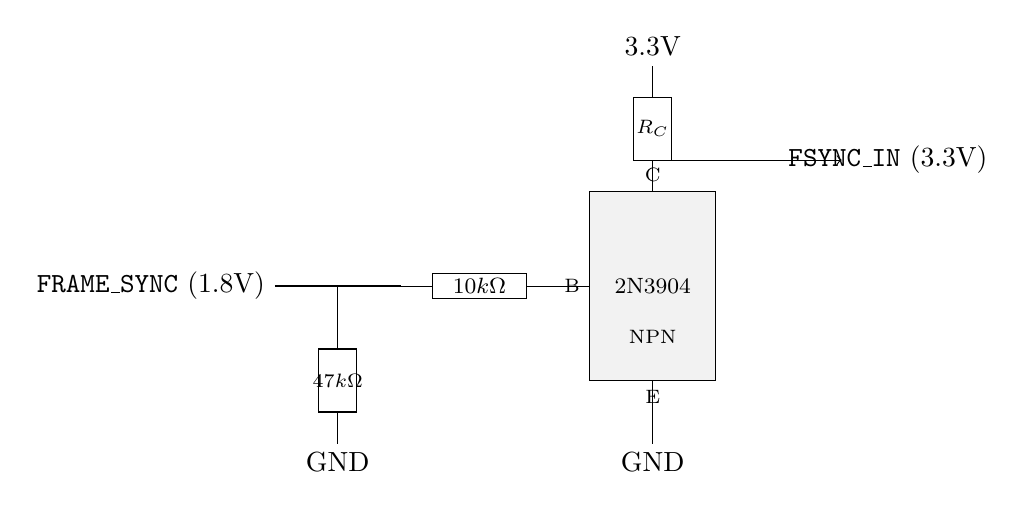
\begin{tikzpicture}[scale=0.8]
        % Signal path
        \node[left] at (0,3) {\texttt{FRAME\_SYNC} (1.8V)};
        \draw[thick] (0,3) -- (2,3);

        % R_base
        \draw (2,3) -- (2.5,3);
        \draw[fill=white] (2.5,2.8) rectangle (4,3.2);
        \node at (3.25,3) {\footnotesize $10\text{k}\Omega$};
        \draw (4,3) -- (5,3);

        % NPN transistor block
        \draw[fill=gray!10] (5,1.5) rectangle (7,4.5);
        \node at (6,3) {\footnotesize 2N3904};
        \node[font=\scriptsize] at (6,2.2) {NPN};

        % Labels
        \node[font=\scriptsize, left] at (5,3) {B};
        \node[font=\scriptsize, above] at (6,4.5) {C};
        \node[font=\scriptsize, below] at (6,1.5) {E};

        % Collector to VCC via R_c
        \draw (6,4.5) -- (6,5);
        \draw[fill=white] (5.7,5) rectangle (6.3,6);
        \node[font=\scriptsize] at (6,5.5) {$R_C$};
        \draw (6,6) -- (6,6.5) node[above] {3.3V};

        % Output from collector
        \draw (6,5) -- (8,5) node[right] {\texttt{FSYNC\_IN} (3.3V)};
        \draw[->] (8,5) -- (9,5);

        % Emitter to GND
        \draw (6,1.5) -- (6,0.5);
        \node at (6,0.2) {GND};

        % Pull-down R
        \draw (1,3) -- (1,2);
        \draw[fill=white] (0.7,1) rectangle (1.3,2);
        \node[font=\scriptsize] at (1,1.5) {$47\text{k}\Omega$};
        \draw (1,1) -- (1,0.5);
        \node at (1,0.2) {GND};
    \end{tikzpicture}
    \caption{NPN transistor level shifter converting 1.8V FRAME\_SYNC to 3.3V logic}
    \label{fig:level_shifter}
\end{figure}

Operation:
\begin{itemize}
    \item When FRAME\_SYNC = 1.8V: Transistor saturates, collector pulled to $\approx$ 3.3V
    \item When FRAME\_SYNC = 0V: Transistor cuts off, base pulled to ground via 47k$\Omega$
\end{itemize}

Rise time is limited by collector capacitance $C_c \approx$ 10 pF and load resistance, yielding $t_r \approx 2.2 \cdot R_C \cdot C_c \approx 230$ ns, negligible relative to 11.1 ms frame interval.

\subsection{FSYNC Distribution}

The synchronized signal fans out to both ESP32 GPIO and IMU FSYNC pin:

\begin{figure}[h]
    \centering
    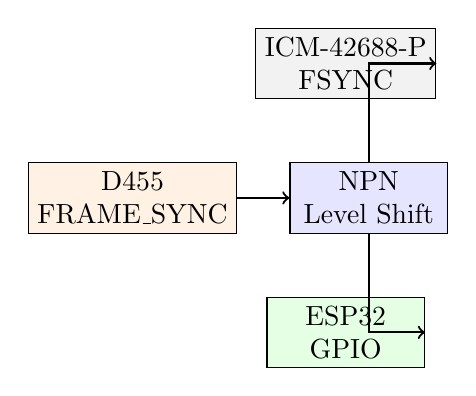
\begin{tikzpicture}[node distance=1cm, auto]
        \node[draw, rectangle, fill=orange!10, minimum width=2cm, minimum height=0.8cm, align=center] (camera) {D455\\FRAME\_SYNC};
        \node[draw, rectangle, fill=blue!10, minimum width=2cm, minimum height=0.8cm, align=center, right of=camera, xshift=2cm] (level) {NPN\\Level Shift};
        \node[draw, rectangle, fill=green!10, minimum width=2cm, minimum height=0.8cm, align=center, below right of=level, yshift=-1cm, xshift=-1cm] (esp32) {ESP32\\GPIO};
        \node[draw, rectangle, fill=gray!10, minimum width=2cm, minimum height=0.8cm, align=center, above right of=level, yshift=1cm, xshift=-1cm] (imu) {ICM-42688-P\\FSYNC};

        \draw[->, thick] (camera) -- (level);
        \draw[->, thick] (level) |- (esp32);
        \draw[->, thick] (level) |- (imu);
    \end{tikzpicture}
    \caption{Synchronization signal distribution topology}
    \label{fig:sync_distribution}
\end{figure}

\section{ESP32 Subsystem}

\subsection{WROOM-32 Module Pinout}

\begin{table}[h]
    \centering
    \caption{ESP32 GPIO assignment}
    \label{tab:esp32_pins}
    \begin{tabular}{lll}
        \toprule
        \textbf{GPIO} & \textbf{Peripheral} & \textbf{Function} \\
        \midrule
        GPIO18 & SPI SCLK & IMU clock \\
        GPIO19 & SPI MISO & IMU data out \\
        GPIO23 & SPI MOSI & IMU data in \\
        GPIO5  & SPI CS   & IMU chip select \\
        GPIO4  & Input    & FSYNC from camera \\
        GPIO15 & Output   & IMU ASSTA reset \\
        GPIO2  & Input    & IMU INT1 data ready \\
        GPIO16 & UART TX  & Debug console \\
        GPIO17 & UART RX  & Debug console \\
        \bottomrule
    \end{tabular}
\end{table}

\subsection{Antenna Design}

The WROOM-32 includes a 2.4 GHz PCB trace antenna with +18 dBm output. For line-of-sight barbell-to-PC transmission (typically 3-8 m), the stock antenna provides sufficient link margin:

\begin{equation}
    P_{rx} = P_{tx} + G_{tx} + G_{rx} - L_{fs} - L_{other}
\end{equation}

where free-space loss $L_{fs} = 20\log_{10}(d) + 20\log_{10}(f) + 32.44$ dB.

At $d = 10$ m, $f = 2.4$ GHz: $L_{fs} \approx 80$ dB. With $P_{tx} = 18$ dBm, $G_{tx} = G_{rx} = 2$ dBi, and ESP32 receive sensitivity of -97 dBm at 1 Mbps, the link margin is 16 dB.

\section{Power Management}

\subsection{Battery Selection}

A 3.7 V LiPo battery powers the entire barbell node. The Apache Pro Mini (3.3V LDO, 500 mA) steps down for logic:

\begin{table}[h]
    \centering
    \caption{Battery runtime estimates}
    \label{tab:battery_runtime}
    \begin{tabular}{lcc}
        \toprule
        \textbf{Capacity} & \textbf{Typical Current} & \textbf{Runtime} \\
        \midrule
        500 mAh & 140 mA & 3.6 hours \\
        1000 mAh & 140 mA & 7.1 hours \\
        2000 mAh & 140 mA & 14.3 hours \\
        \bottomrule
    \end{tabular}
\end{table}

\subsection{Charging Circuit}

The TP4056 linear charger provides 1 A constant-current/constant-voltage charging with 4.2 V termination. Protection features include:
\begin{itemize}
    \item Over-current protection at 1.5 A
    \item Thermal regulation during high ambient temperature
    \item Automatic recharge when cell voltage drops below 4.05 V
\end{itemize}

\section{PCB Design Considerations}

\subsection{Layer Stackup}

A 4-layer stackup is recommended for RF performance:

\begin{enumerate}
    \item Top: Components + signal routing
    \item Layer 2: Ground plane (solid)
    \item Layer 3: Power plane (3.3V + 1.8V regions)
    \item Bottom: Signal routing + antenna trace
\end{enumerate}

\subsection{Impedance Control}

The ESP32 antenna trace requires 50$\Omega$ characteristic impedance. For a microstrip on FR-4 ($\epsilon_r \approx 4.3$):

\begin{equation}
    Z_0 \approx \frac{87}{\sqrt{\epsilon_r + 1.41}} \ln\left(\frac{5.98h}{0.8w + t}\right)
\end{equation}

With $h = 0.2$ mm (dielectric thickness), $w = 0.4$ mm (trace width), $t = 0.035$ mm (copper), $Z_0 \approx 51\Omega$.

\section{Mechanical Integration}

\subsection{Barbell Mounting}

The sensor node mounts on the barbell collar using a 3D-printed (PLA) enclosure with:
\begin{itemize}
    \item Radial symmetry to minimize barbell imbalance (<5 g asymmetry)
    \item Securing mechanism compatible with standard Olympic collars
    \item IP54-rated enclosure to resist chalk dust and sweat
    \end{itemize}

The total added mass is 42 g, concentrated at the sleeve end 730 mm from bar center, producing moment of inertia increase of $m r^2 = 0.042 \cdot 0.73^2 \approx 22$ g$\cdot$m\textsuperscript{2}, negligible compared to a loaded barbell's $\approx 5$ kg$\cdot$m\textsuperscript{2}.

\section{PCB Fabrication Specifications}

\begin{table}[h]
    \centering
    \caption{PCB fabrication notes}
    \label{tab:pcb_specs}
    \begin{tabular}{ll}
        \toprule
        \textbf{Parameter} & \textbf{Specification} \\
        \midrule
        Substrate & FR-4 TG-150 \\
        Thickness & 1.6 mm $\pm$ 0.1 mm \\
        Copper Weight & 1 oz (35 $\mu$m) \\
        Min Trace/Space & 4/4 mil \\
        Solder Mask & Green, nominal 20 $\mu$m \\
        Surface Finish & ENIG (immersion gold) \\
        Impedance Control & 50$\Omega$ $\pm$10\% \\
        \bottomrule
    \end{tabular}
\end{table}

\section{Summary}

This chapter detailed the hardware implementation including IMU configuration, synchronization circuitry, ESP32 interfacing, power management, and mechanical integration. The design achieves sub-200 $\mu$s synchronization accuracy while maintaining portability and battery autonomy suitable for extended training sessions.

\newpage